% ------------------------------------------------------------- 
% Arquivo :  relatório modelo                                        
% ------------------------------------------------------------- 
% O percentual(%) serve para incluir comentários: 
% tudo o que fica à direita dele não é interpretado pelo LaTex
% Linhas e espaços em branco também **NÃO** são
% interpretadas pelo LaTex

%% As intruções seguintes são o cabeçalho e devem estar antes do
%% \begin{document}

%\documenclass: mandatorio, indica o tipo/formato de documento
\documentclass[brazilian,12pt,a4paper,final]{article}
% tamanhos de fontes: 10pt, 11pt ou 12pt
% opções de estilo (padrões): article, report, book, slide, letter (artigo, relatorio, livro, apresentação de slides, carta)




%% Pacotes extras (opcionais):

% *babel* contem as regras de ifenização
\usepackage[brazil]{babel}

% *t1enc* permite o reconhecimento dos acentos inseridos com o teclado
%\usepackage{t1enc}

% *inputenc* com opção *utf8* permite reconhecimento dos caracteres com codificação UTF8, que é padrão dos esditores de texto no Linux. Isso permite reconhecimento automático de acentuação.
\usepackage[utf8]{inputenc}


% *graphicx* é para incluir figuras em formato eps 
\usepackage{graphicx} % para produzir PDF diretamente reescrever esta linha assim: \usepackage[pdftex]{graphicx}

% *color* fontes soloridas
\usepackage{color}
%%% fim do cabecalho %%%

\pagestyle{empty}
\title{Métodos Computacionais da Física A}
\author{Aluno: Átila Leites Romero \\ Matrícula: 144679 \\ IF-UFRGS}

\begin{document}
\maketitle
\begin{abstract}
Verificação experimental da lei de Murphy para torradas amanteigadas.
\end{abstract}

\section{Introdução} 
%Pequeno histórico do problema. 
%Explicar porque o trabalho é relevante.
Uma das leis de Murphy diz que se algo pode dar errado, dará errado.
Aplicada ao cotidiano matinal, esta lei foi adaptada e, hoje,
é de conhecimento popular  que as torradas sempre caem com a parte
amanteigada virada para baixo.

Neste trabalho será verificada a veracidade desta hipótese.

\section{Método}
% Aqui o Método 
%Detalhes sobre o método utilizado \cite{Kauffman_book},
%procure ao final do texto a referencia a esta bibliografia.
%demonstrações de porque ele funciona.  Limites analíticos, etc.
Para montagem da experiência, foram utilizados:
\begin{enumerate}
  \item{ Pacote de pão de forma }
  \item{Torradeira}
  \item{Tablete de manteiga}
  \item{Faca}
  \item{Cobaia}
\end{enumerate}

Inicialmente, os pães foram inseridos em duplas na torradeira. Em 
seguida, as torradas resultates foram embaralhadas e metade delas foi separada para
servir de grupo controle.

Cada torrada do grupo de teste teve um lado preenchido com manteiga.

Como uma parte importante da hipótese atesta que algo deve poder dar errado, é 
fundamental a utilização da cobaia, 

Exemplo de fórmula matemática:
\mbox{}

$$ \int_{0}^{\infty} f(x) dx $$

\vspace{0.5cm}

Exemplo de lista numerada:
\begin{enumerate}
  \item{ primeiro }
  \item{ etc }
  \item{ etc }
\end{enumerate}

% O verbatim faz o latex ignorar a formatação: ai SIM os espaços e
% linhas em branco contam
% É util para trechos de código Fortran por exemplo
\vspace{0.3cm}
Exemplo de texto sem formatação para código {\bf FORTRAN} por exemplo
Veja o %\bf acima

\begin{verbatim}
...
Read (*,*) a, b, t

 Do i=0,t
    b(i) = a*c(i)
 End do
...

\end{verbatim}

\section{Resultados}
\vspace{2cm}
 Aqui os resultados, sua interpretação.

% Aqui incluimos uma figura
% Para testar este comando devem criar uma figura em formato
% postscript encapsulado (eps) e deve ter o mesmo nome que aparece entre chaves
% no caso ``fig.eps'' 
Incluindo uma figura em formato {\it eps}

\begin{figure}[hbtp]
\begin{center}
\includegraphics[width=8cm]{figura.eps}
\caption{Coloque aqui as legendas}
\label{fig}
\end{center}
\end{figure}
\vspace{0.5cm}

\begin{figure}[htbp]
\begin{center}
\rotatebox{-90}{\resizebox{8.0cm}{!}{\includegraphics{figura.eps}}}
\caption{Legendas}
\label{fig_rotacao}
\end{center}
\end{figure}



Incluindo uma tabela:
\begin{table}[h]
\begin{tabular}{||l|c|r||} \hline
tempo& posição & velocidade\\
\hline
 0 & 1 & 3\\
 1 & 2 & 4\\
 2 & 3 & 5\\
 \hline
 \end{tabular}
 \caption{A tabela mostra os valores de tempo, posiçao e velocidade do
{\ldots} }
\end{table}

\section{Conclusões}
Recolocar resumidamente o problema, os resultados, as comparações \cite{Wolfram_book} com outros
trabalhos e as perspectivas futuras que o trabalho abre.

{\color{red} Este é um modelo geral, quando for utilizá-lo para um trabalho
específico leve em consideração as necesidades desse trabalho,
cuidando de omitir ou comentar com \% \% as seções que não
se apliquem.}

\begin{thebibliography}{99}

\bibitem{Kauffman_book}
S.~Kauffman, {\em The Origins of Order: Self-Organisation and
Selection in Evolution}, (Oxford University Press, 1993).

\bibitem{Wolfram_book}
S.~Wolfram, {\em Theory and Application of Cellular Automata},
(World Scientific, Singapore, 1986).

\end{thebibliography}

\end{document}

